
\subsection{Lewin's Force Field Analysis}

	{A force field analysis was used to analyze the driving and restraining forces so as to decide whether DDE should consider outsourcing. Each force factor is ranked out of 5 in terms of significance and net sums of both the forces are calculated and compared to determine whether the change should occur.}
	
	\begin{figure}[H]
    	\centering
    	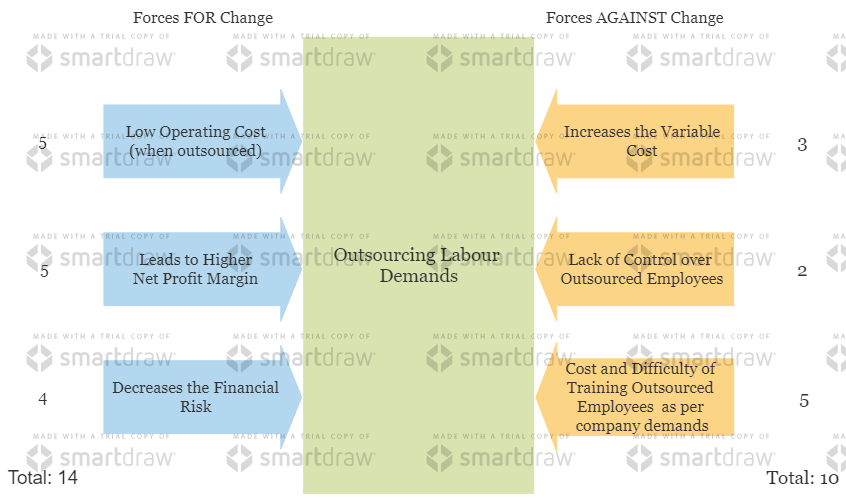
\includegraphics[width=15cm]{Lewin's Force Analysis.png}
    	%\caption{{Lewin's Force Field Analysis of the problem the company is facing}}
    	\label{}
	\end{figure}
	
	{}	

\subsection{Ratio Analysis}

	{Ratio Analysis is a numerical and qualitative financial tool that can be used to determine the current and future financial position of DDE for if the company can consider outsourcing its labour demands.}

%	\noindent
%	% Gross Prift Margin (Current)
%	\begin{minipage}{.5\linewidth}
%	\begin{equation}
%		\frac{\text{Current Gross Proft}}{\text{Current Revenue}}\times 100 \%
%	\end{equation}
%	\end{minipage}
%	% Gross Profit Margin (Future)
%	\begin{minipage}{.5\linewidth}
%	\begin{equation}
%		\frac{\text{Predicted Gross Proft}}{\text{Predicted Revenue}}\times 100 \%
%	\end{equation}
%	\end{minipage}

	%	Gross Profit Margin (Current)

	$$\text{Gross Profit Margin (Current)} = \frac{\text{Current Gross Proft}}{\text{Current Revenue}}\times 100\% = \frac{\$1296000}{\$2160000}\times 100\% = 60\%$$

	%	Gross Profit Margin (Future)

	$$\text{Gross Profit Margin (Future)} = \frac{\text{Predicted Gross Proft}}{\text{Predicted Revenue}}\times 100\% = \frac{\$2333000}{\$3888000}\times 100\% \approx 60.2\%$$
	
	%	Net Profit Margin (Current)

	$$\text{Net Profit Margin (Current)} = \frac{\text{Current Net Profit}}{\text{Current Revenue}}\times 100\% = \frac{\$705375}{\$2160000}\times 100\% \approx 32.7\%$$
	
	%	Net Profit Margin (Future)

	$$\text{Net Profit Margin (Future)} = \frac{\text{Predicted Net Profit}}{\text{Predicted Revenue}}\times 100\% = \frac{\$1995000}{\$3888000}\times 100\% \approx 51.3\%$$
	
	%	Current Ratio (Only for Current)

	$$\text{Current Ratio} = \frac{\text{Current Assets}}{\text{Current Liabilities}} = \frac{\$600000}{\$245000} \approx 2.45$$
	
	%	Return on Capital Employed (Current)

	$$\text{Return on Capital Employed (Current)} = \frac{\text{NPBIT}}{\text{Capital Employed}}\times 100\% = \frac{\$897500}{\$699300}\times 100\% \approx 128\%$$
	
	%	Return on Capital Employed (Future)

	$$\text{Return on Capital Employed (Future)} = \frac{\text{NPBIT}}{\text{Capital Employed}}\times 100\% = \frac{\$2256000}{\$1731000}\times 100\% \approx 130\%$$

	{The Gross Profit Margin for both the company's current and predicted financial state (if the company is to decide to outsource its labour) are both relatively healthy and above the optimal $50\%$ range. This shows the company is profitable and has no issues with the lack of profitability. This statement is further supported by a very good Net Profit Margin of $32.7\%$ before considering outsourcing and an excellent predicted Net Profit Margin of $51.3\%$ after outsourcing.}
	
	{When analyzing the business Profit-Loss accounts, it is evident that other than the cost of revenue before outsourcing, the operating cost is relatively very high, whereas the operating cost after outsourcing is reduced significantly and is fraction of the original operating cost.}
	
	{The current ratio is largely positive, demonstrating that the company is in a healthy and stable Cash-Flow position and would not be at a financial risk if the company is to start outsourcing their labour demands.}	
	
	{We can confidently say from the above conclusions that the company can  increase their firm's growth and profit margin by outsourcing labour.}

\subsection{SWOT Analysis}

	{}
	
	\begin{figure}[H]
    	\centering
    	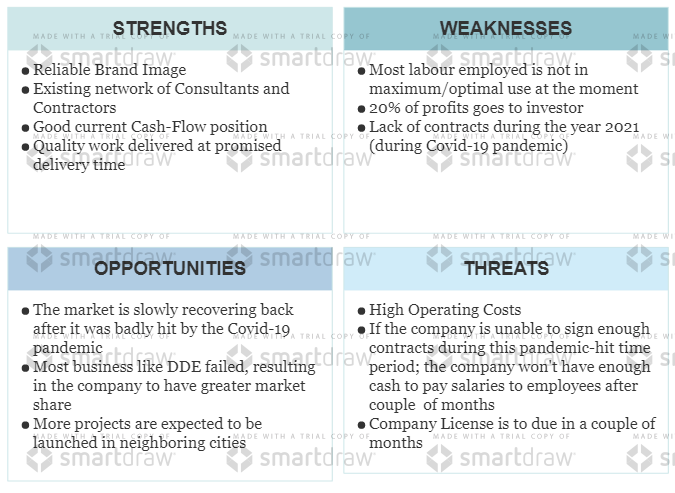
\includegraphics[width=15cm]{SWOT Analysis.png}
    	%\caption{{SWOT Analysis of the problem the company is facing}}
    	\label{}
	\end{figure}

	{}	

\subsection{Fishbone Diagram}

	{The Fishbone diagram finds and analyses the root issue/problem faced within a business. This business tool shall determine the underlying problems/reasons faced by DDE causing the company to consider outsourcing. The main concern from the owner of the firm is Lower Profit Margin.}
	
	\begin{figure}[H]
    	\centering
    	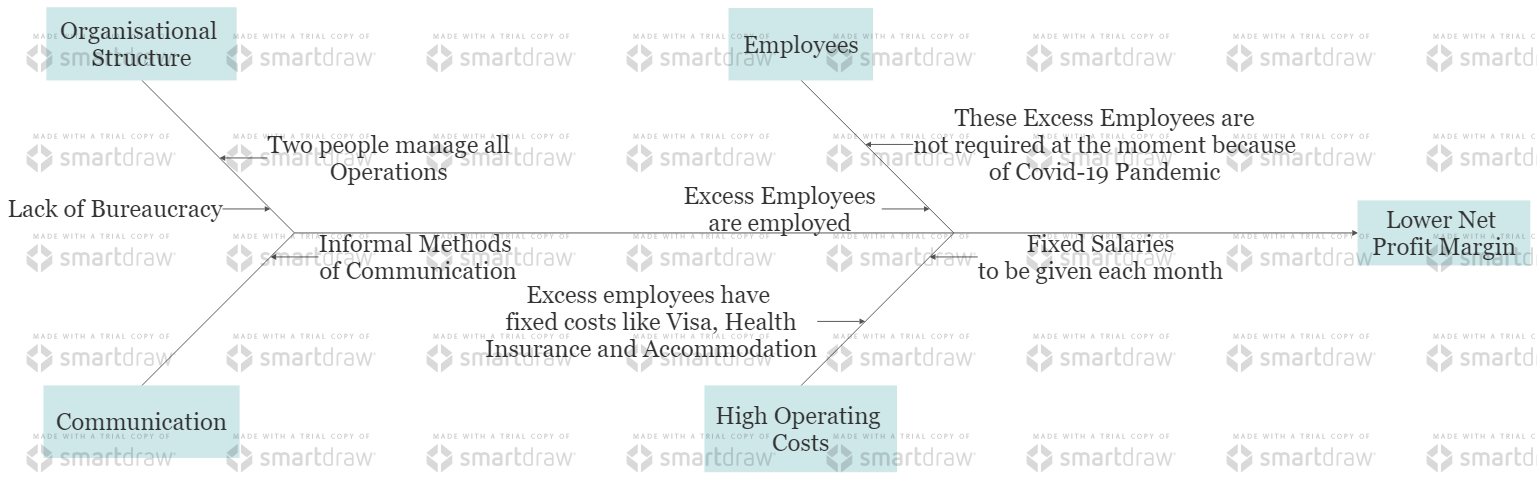
\includegraphics[width=15cm]{Fishbone Diagram.png}
    	%\caption{{Fishbone Diagram of the problem the company is facing}}
    	\label{}
	\end{figure}

	{}
	
	{}
	
	{}

\subsection{PEST Analysis}

	{}

